% Source: Code/xband-radar-sim/docs/radar_simulation_technical.tex
% Description: Effect of windowing on pulse compression. Hamming window reduces sidelobes from -13 dB to -42 dB.

\documentclass[border=4pt]{standalone}
\usepackage{algpseudocode}
\usepackage{amsmath,amssymb,amsfonts}
\usepackage[T1]{fontenc}
\usepackage{graphicx}
\usepackage{pgfplots}
\usepackage{tikz}
\usepackage{xcolor}
\pgfplotsset{compat=1.18}
\usetikzlibrary{arrows.meta,positioning,shapes.geometric,calc,patterns,decorations.pathmorphing,3d,angles,quotes}

\definecolor{radargreen}{RGB}{0,255,0}
\definecolor{raycolor}{RGB}{255,165,0}
\definecolor{targetcolor}{RGB}{255,0,0}
\definecolor{groundcolor}{RGB}{139,90,43}
\definecolor{skycolor}{RGB}{135,206,235}
\definecolor{beamcolor}{RGB}{255,255,0}


\begin{document}
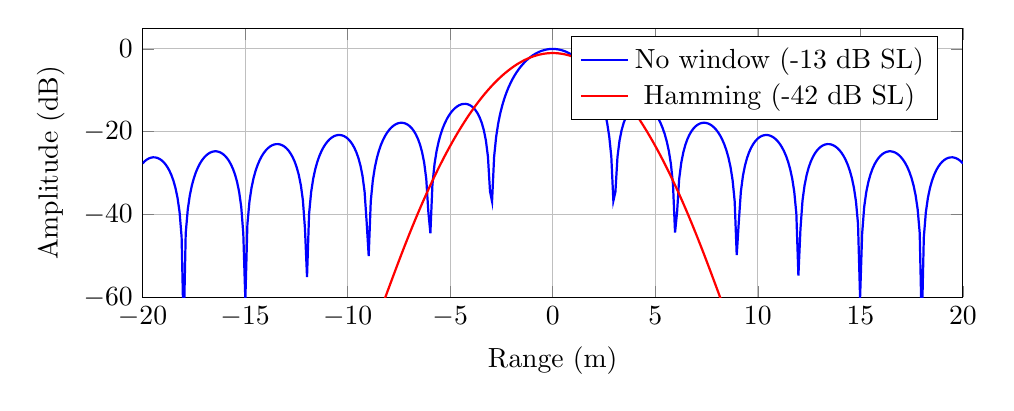
\begin{tikzpicture}
\begin{axis}[
    width=12cm, height=5cm,
    xlabel={Range (m)},
    ylabel={Amplitude (dB)},
    xmin=-20, xmax=20,
    ymin=-60, ymax=5,
    grid=both,
    legend pos=north east
]
    % Unwindowed (sinc)
    \addplot[thick, blue, domain=-20:20, samples=400] {
        20*log10(abs(sin(deg(pi*x/3))/(pi*x/3 + 0.0001)) + 0.0001)
    };
    \addlegendentry{No window (-13 dB SL)}

    % Windowed (approximation)
    \addplot[thick, red, domain=-20:20, samples=400] {
        20*log10(exp(-0.5*(x/2.2)^2) + 0.0001) - 1
    };
    \addlegendentry{Hamming (-42 dB SL)}

\end{axis}
\end{tikzpicture}
\end{document}
